\documentclass[a4paper]{article}
\usepackage{graphicx}   % Para insertar graficos
\usepackage{titling}    % Titulo y caratula
\usepackage{float}      % Para el argumento H en las figuras
\usepackage{wrapfig}    % wrapfigures
\usepackage{subcaption} % Subfigures
\usepackage[left=2cm,right=2cm,top=2cm,bottom=2cm]{geometry}

\graphicspath{ {graficos/} }

\pretitle{\noindent\rule{\textwidth}{2pt}\bigskip\begin{center}\LARGE\bfseries}
\posttitle{\end{center}\bigskip\noindent\rule{\textwidth}{2pt}}
\preauthor{\vspace*{2cm}\begin{center}\LARGE}
\postauthor{\end{center}}
\predate{\vspace*{10cm}\begin{center}\Large}
\postdate{\end{center}}

% TODO Agregar universidad, y algo mas
\title{
  Probabilidad y Estadistica\\
  Trabajo Practico - Estadistica Descriptiva
}
\author{Peirone Bautista, Scola Luciano}
\date{Abril, 2023}
\begin{document}
\begin{titlepage}
\maketitle
\thispagestyle{empty} % No cuenta la portada para el numero de paginas
\end{titlepage}
\newpage

\section{Introducción} % Este es la descripcion del problema, hay que adaptarlo a la intro.
La contaminaci ́on del aire representa un importante riesgo medioambiental para la salud. Se esti-
ma que, en los pa ́ıses menos desarrollados, cerca de la tercera parte de las muertes y enfermedades

se deben directamente a causas ambientales. Un ambiente m ́as saludable permitir ́ıa reducir con-
siderablemente la incidencia de c ́anceres, enfermedades cardiovasculares, asma, infecciones de las

v ́ıas respiratorias, entre otros padecimientos que producen millones de muertes por a ̃no. Esto re-
presenta actualmente uno de los mayores riesgos sanitarios mundiales, comparable con el tabaco

y s ́olo superado por los riesgos sanitarios relacionados con la hipertensi ́on y la nutrici ́on.
Ahora bien, los  ́arboles en general, y el arbolado urbano en particular, cumplen un papel relevante
en la lucha contra la contaminaci ́on del aire. En principio, reducen dicha contaminaci ́on porque
absorben los componentes gaseosos t ́oxicos, principalmente el CO2, al que transforman en ox ́ıgeno
para su posterior liberaci ́on a la atm ́osfera. Paralelamente, este proceso transformador de CO2
es mencionado en el Protocolo de Kyoto como el motor de la reducci ́on del calentamiento global
y del efecto invernadero. Particularmente, hay  ́arboles y arbustos que reducen la contaminaci ́on
interceptando peque ̃nas part ́ıculas del aire, otros que atraen insectos que favorecen la polinizaci ́on,
as ́ı como tambi ́en hay especies que sombrean mayores superficies propiciando un descenso de la
temperatura urbana.
Por los motivos enunciados, en el a ̃no 2011 se realiz ́o un Censo Forestal Urbano P ́ublico en dos
comunas del sur de Buenos Aires, con el objetivo de contabilizar y determinar el estado actual del
arbolado urbano p ́ublico.

Las fuentes para los datos usadas en este trabajo provienen del Censo Forestal
Urbano Público realizado en la ciudad de Buenos Aires en el año 2011, y todos
los análisis que se harán de aquí en más se basan en esta fuente.

Finalmente, se dará una conclusión general sobre el análisis hecho y los datos.

\section{Objetivo}
El objetivo de este informe es presentar un análisis acerca de datos recopilados
sobre el arbolado urbano en la ciudad de Buenos Aires en el año 2011, con el
fin de proveer al lector de una idea general de este y relacionarlo con la
problemática que en su momento dio lugar a la necesidad de recopilar estos datos,
la contaminación del aire en la ciudad.

\newpage

\section{Desarrollo}
Los datos sobre los cuales se trabaja en este informe proveen información acerca
de distintos aspectos de una muestra tomada del arbolado urbano en Buenos Aires.
Tales aspectos son: altura, inclinación, diámetro, especie, origen
y cantidad de brotes en el ultimo año. Se observa que la altura está dada en metros(m),
la inclinación en grados(°) y el diámetro en centímetros(cm).

A lo largo del trabajo, nuestro objeto de interés serán arboles de la muestra,
por lo que la unidad de análisis serán arboles, y se analizaran tanto los aspectos
y características de los arboles por separado tanto como análisis bivariados de estos.

% Rellenar con algo mas capaz
\subsection{Altura}

La altura es un factor clave en los árboles, principalmente en situación urbana y
es de gran importancia para la sombra que produce un árbol, donde gran cantidad de
arboles altos tienden a disminuir la temperatura de una ciudad.

Esta variable es de naturaleza cuantitativa continua, porque representa una medición,
y presenta un cero absoluto.
Se presenta el siguiente histograma.

\begin{figure}[H]
    \centering
    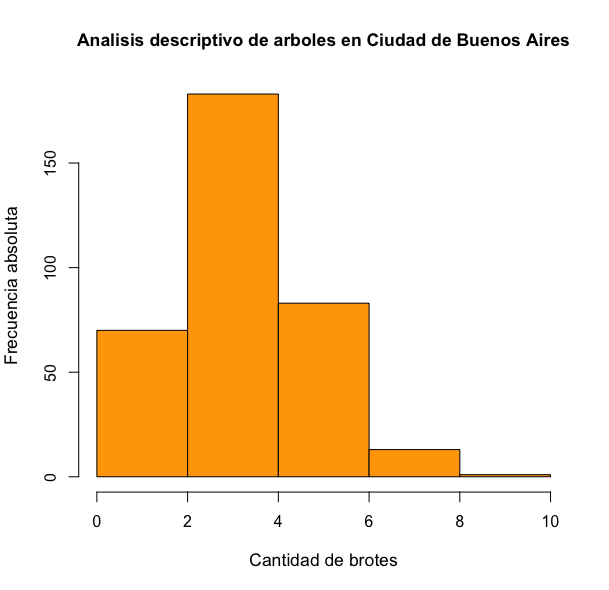
\includegraphics[width=\textwidth]{altura/histograma.png}
    \caption{Ejemplo de histograma}
    \label{fig:histograma altura}
\end{figure}
\begin{figure}[H]
    \centering
    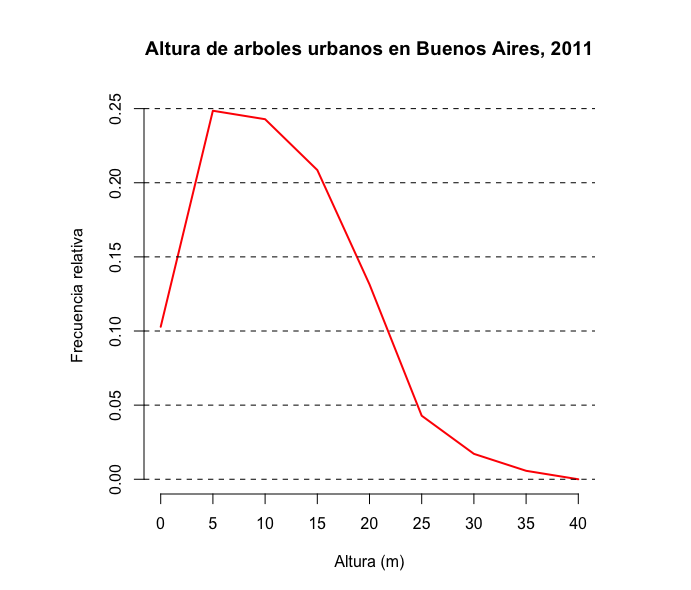
\includegraphics[width=\textwidth]{altura/poligono frecuencia.png}
    \caption{Polígono de frecuencias}
    \label{fig:poligono frecuencia altura}
\end{figure}
\begin{figure}[H]
    \centering
    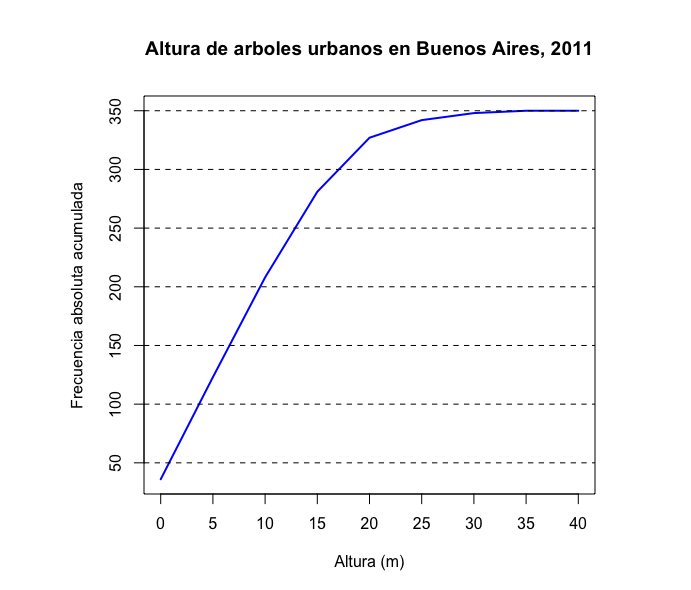
\includegraphics[width=\textwidth]{altura/poligono acumulativo.png}
    \caption{Polígono de frecuencias}
    \label{fig:poligono acumulativo altura}
\end{figure}

En la figura \ref{fig:histograma altura} se puede observar la distribución de las alturas de
los arboles en la muestra, donde se observa que la mayoría de arboles se encuentran en
el rango de 5 a 20 metros de altura.

Puntualmente, en la figura \ref{fig:poligono altura} se observa la frecuencia relativa
de estas.

\subsection{Diámetro}
En esta sección se da un análisis general del diámetro de los arboles en la muestra.
Se presenta el siguiente gráfico. El diámetro es una variable cuantitativa continua y
con un cero absoluto, ya que representa una medición de un aspecto físico. En las fuentes
usadas, los diámetros han sido redondeados a números enteros.

\begin{figure}[H]
    \centering
    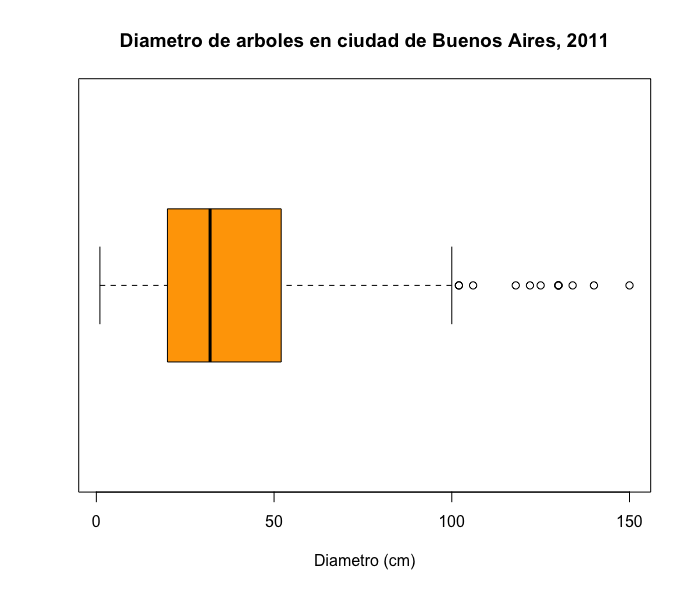
\includegraphics[width=\textwidth]{diametro/boxplot.png}
    \caption{Grafico de caja de diametros}
    \label{fig:boxplot diametro}
\end{figure}
Del gráfico \ref{fig:boxplot diametro} de caja se pueden obtener las siguientes conclusiones:
La mediana del diámetro de los arboles en la muestra es aproximadamente 30 cm, con primer y
segundo cuartil de 20 cm y 50 cm respectivamente. Hay varios valores outliers por derecha,
y el máximo valor de diámetro que no es outlier corresponde con 100 cm, mientras que el
valor mínimo es de 1 cm.

\subsection{Inclinación}
La inclinación de los arboles en la muestra han sido medidos en ángulos (°). Esta variable
es cuantitativa continua, representando el ángulo que forma el tronco del árbol con una
perpendicular del suelo. Sin embargo, por la naturaleza de esta y la forma en que se
encuentra en la fuente, se ha decidido mostrar esta variable en terminos de dos posibles
categorias: Muy inclinado, poco inclinado, donde cada una representa...

\subsection{Origen}
El origen de un árbol es una variable categórica, con dos posibles categorías en la muestra,
exótico o nativo/autóctono.
De acuerdo a la figura \ref{sfig:pie origen}, la cantidad de arboles exóticos en la muestra es
superior a la de arboles nativos.

Mas detalladamente, el gráfico \ref{sfig:barplot origen} presenta las frecuencias absolutas con
que sucede cada posible origen, teniendo casi 250 ejemplares exóticos en la muestra, contra tan
solo aproximadamente 120 arboles nativos.

\begin{figure}
    \centering
    \caption{Porcentajes de origen}
    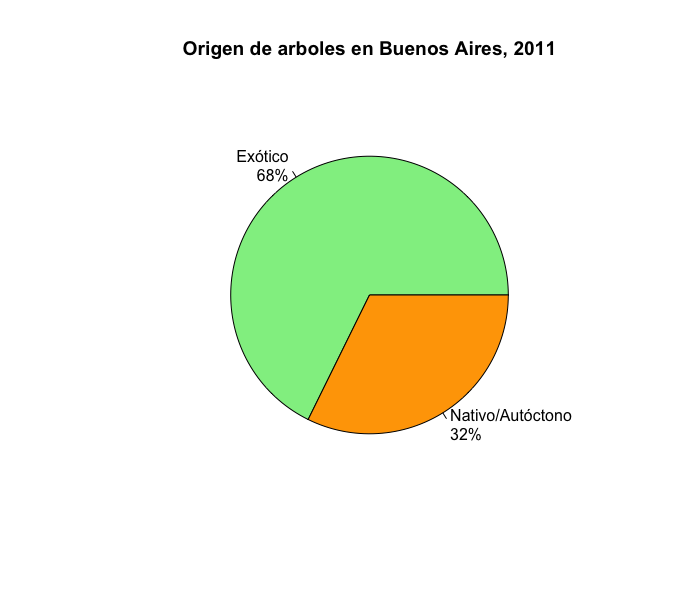
\includegraphics[width=\textwidth]{origen/pie.png}
    \label{sfig:pie origen}
\end{figure}
\begin{figure}[H]
    \centering
    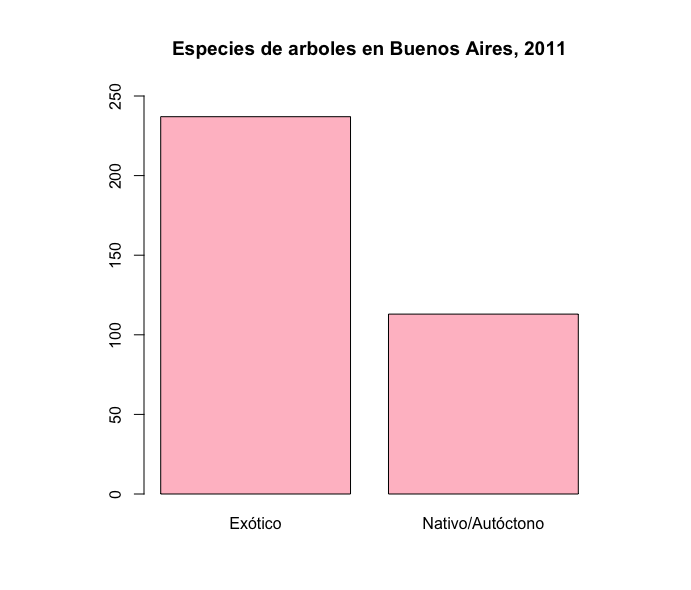
\includegraphics[width=\textwidth]{origen/barplot.png}
    %\caption{}
    \label{fig:barplot especie}
\end{figure}

\subsection{Especie}
La especie de un árbol es una variable categórica. Sobre los datos analizados se distinguen
9 especies distintas.

Se observa que la moda de especies es el eucalipto, con más de 80 eucaliptos en la muestra.

\subsection{Brotes}
\begin{figure}[H]
    \centering
    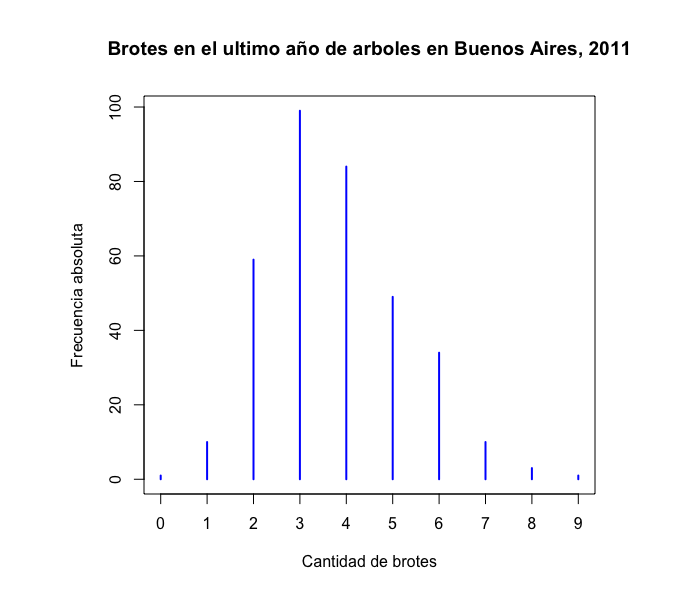
\includegraphics[width=\textwidth]{brotes/bastones.png}
    \caption{Frecuencia absoluta de cantidad de brotes en el ultimo año}
    \label{fig:bastones brotes}
\end{figure}
\begin{figure}[H]
    \centering
    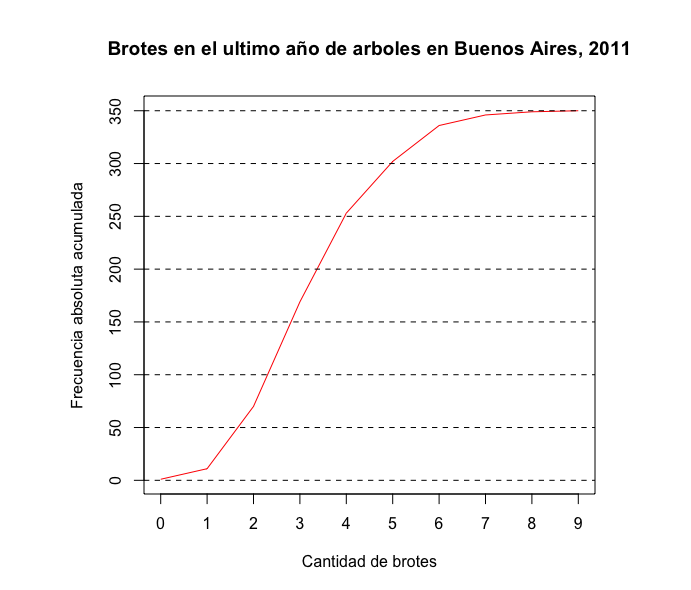
\includegraphics[width=\textwidth]{brotes/poligono acumulado.png}
    \caption{Frecuencia absoluta acumulada de cantidad de brotes en el ultimo año}
    \label{fig:poligono acumulado brotes}
\end{figure}

\subsection{Bivaridado}
El fin de esta sección es describir la relación entre dos variables de las ya estudiadas
con anterioridad en secciones pasadas.

\begin{center}
  \begin{table}[ht]
    \centering
    \begin{tabular}{rrrrrrrrrr}
      \hline
      & Acacia & Álamo & Casuarina & Ceibo & Eucalipto & Ficus & Fresno & Jacarandá & Palo borracho \\ 
      \hline
      [0,5) &   2 &   2 &   1 &   4 &   1 &   4 &   3 &   5 &   5 \\ 
      [5,10) &   9 &  12 &   5 &   5 &   2 &   3 &  11 &  11 &  14 \\ 
      [10,15) &   3 &  13 &  14 &   3 &   8 &   1 &  19 &  10 &  14 \\ 
      [15,20) &   5 &  11 &  10 &   4 &  12 &   4 &   8 &  15 &  16 \\ 
      [20,25) &   0 &   7 &   4 &   0 &  32 &   0 &   2 &   0 &   3 \\ 
      [25,30) &   0 &   3 &   1 &   0 &  15 &   0 &   0 &   1 &   0 \\ 
      [30,35) &   0 &   0 &   0 &   0 &  10 &   0 &   0 &   0 &   0 \\ 
      [35,40) &   0 &   0 &   0 &   0 &   3 &   0 &   0 &   0 &   0 \\ 
      \hline
    \end{tabular}
  \end{table}
\end{center}


\section{Conclusión}

\end{document}
